\documentclass[12pt]{article}
\usepackage[utf8]{inputenc}
\usepackage{amsmath}
\usepackage{fancyhdr}
\usepackage{graphicx}
\usepackage{epstopdf}

\setlength{\oddsidemargin}{0in}
\setlength{\evensidemargin}{0in}
\setlength{\textwidth}{6.5in}
\setlength{\topmargin}{-.3in}
\setlength{\textheight}{9in}


\pagestyle{fancy}
\begin{document}

\begin{center}
{\Large Machine Learnig Homework } \\[.3in]
\end{center}
\lhead{Adam Kosiorek}
\rhead{IMAT: 03661883}
\vspace*{.5in}


\section*{Problem 1}

Let us assume without any loss of generality that $y > x$. Since $t \in ]0, 1[$ we see that $tx + (1-t)y = z \in ]x, y[$. Therefore, the definition of a strictly convex function does not consider the function's graph at points $x$ and $y$. A graph of strictly convex function must lie strictly below a straight line from $f(x)$ to $f(y)$ and $f$ cannot be linear \emph{e.g.} $f(x) = ax + b$ . It is different from a convex function, whose graph can be a straight line.

\section*{Problem 2}

If a function is convex, it can be a straight line $f(x) = ax + b$. Since $a$ can be equal to $0$, the function $f(x) = b$ is a convex function for which $\forall_{x \in \mathcal{R}} f(x) = b$. Therefore an infinite number of points $x^*$ satisfies $x^* = \arg \min_x f(x)$.

\section*{Problem 3}

If a function $f$ is strictly convex, the graph of $f$ must lie below a straight line between points $(x, f(x))$ and $(y, f(y))$ for any $x \neq y$. We know that $\nabla f(x^*) = 0$. Let's take a point $x_0$ such that $y = c$ for some constant $c$ is a horizontal line that crosses $f(x)$ at the point $x_0$. We know that at least a part of the graph of $f$ must lie below the line $y = c$. We can move this line to a point just above $f(x^*)$ such that $f(x^*)$ is the only point below the line. Therefore, there is only a single point that satifies $f(x^*) = min_x f(x)$ for a strictly convex function f.

\section*{Problem 4}

\begin{figure}[!ht]
  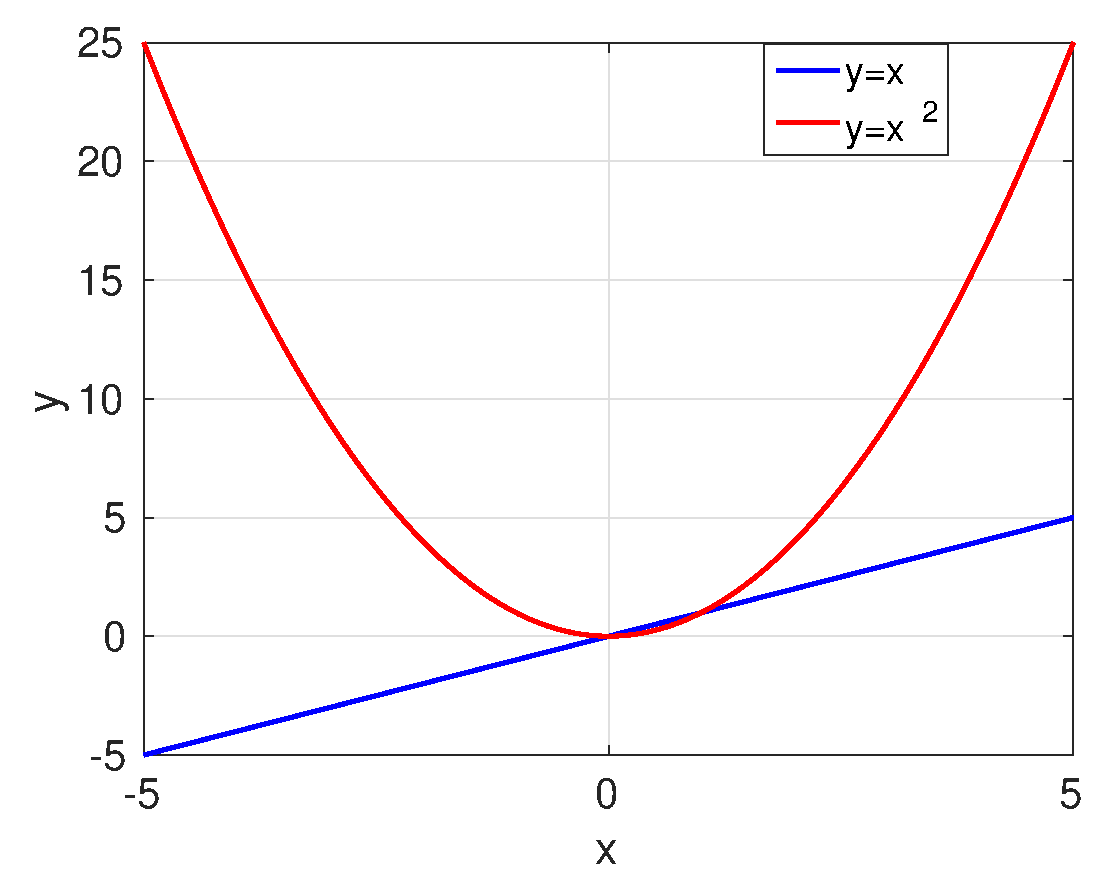
\includegraphics[width=\linewidth]{convex}
  \caption{An example of a strictly convex function $y = x^2$ and a non-strictly convex function $y = x$.}
  \label{fig:convex}
\end{figure}

As in Fig. \ref{fig:convex}.
  
\section*{Problem 5}

We cannot apply this feature to data directly. It is infinite dimensional and would require infinite memory to store and time to compute.

\section*{Problem 6}

\begin{equation}
\begin{align}
 K(x, y) &= \sum_{i=1}^\infty \phi_{\infty, i}(x)\phi_{\infty, i}(y) \\
	 &= \sum_{i=1}^\infty \frac{1}{i!} e^\frac{-(x^2 + y^2)}{2 \sigma^2} \left( \frac{xy}{\sigma^2} \right)^i \\
	 &= e^\frac{-(x^2 + y^2)}{2 \sigma^2} \sum_{i=1}^\infty \frac{1}{i!} \left( \frac{xy}{\sigma^2} \right)^i \\
	 &= e^\frac{-(x^2 + y^2)}{2 \sigma^2} \sum_{i=1}^\infty \frac{1}{i!} \left( z \right)^i
 \end{align}
\end{equation}

where $z = \frac{xy}{\sigma^2}$. From the Taylor expansion of $e^z$ around $0$ we have

\begin{equation}
  e^z = 1 + z + \frac{1}{2!} z^2 + \ldots = 1 + \sum_{i=1}^\infty \frac{1}{i!} z^i
\end{equation}

and therefore $\sum_{i=1}^\infty \frac{1}{i!} z^i = e^z - 1$. Finally

\begin{equation}
\begin{align}
 K(x, y) &= e^\frac{-(x^2 + y^2)}{2 \sigma^2} \left( e^\frac{xy}{\sigma^2} - 1 \right) \\
         &= e^\frac{-(x - y)^2}{2 \sigma^2} - e^\frac{-(x^2 + y^2)}{2 \sigma^2}
\end{align}
\end{equation}

which is easy to compute. We should be concerned with overfitting, since an infinite dimensional feature space translates to very high complexity of the model. It can fit training data perfectly, but generalize badly. It is at least partially mitigated by SVM, because it looks for a large margin decision boundary, which improves generalization.      


\section*{Problem 7}

For every $x, y$ it holds that $x^2 + y^2 \geq (x - y)^2$ which implies that $e^\frac{-(x - y)^2}{2 \sigma^2} \geq e^\frac{-(x^2 + y^2)}{2 \sigma^2}$ and $K(x, y) \geq 0$. A linear decision boundary is given by $f(x) = w^T \phi_\infty(x)$ where the parameters $w$ are given by a linear combination of training examples $w = \sum_{i=1}^N \alpha_i y^{(i)} \phi_\infty(x^{(i)})$, where $y^{(i)} \in \{0, 1\}$ is label of the $i^{th}$ data sample. We have 

\begin{equation}
 \begin{align}
  f(x^{(j)}) &= \sum_{i=1}^N \alpha_i y^{(i)} \phi_\infty(x^{(i)})^T \phi_\infty(x^{(j)}) \\
       &= \sum_{i=1}^N  \alpha_i y^{(i)} K(x^{(i)}, x^{(j)}) \\
       &= \sum_{i=1}^N  \alpha_i y^{(i)} \left( e^\frac{-\left(x^{(i)} - x^{(j)}\right)^2}{2 \sigma^2} - e^\frac{-\left(\left(x^{(i)}\right)^2 + \left(x^{(j)}\right)^2\right)}{2 \sigma^2} \right)
 \end{align}
\end{equation}

Let $\alpha_i = 1$ for every $i$ and set $\sigma = 10^{-6} \min_{i, j} \left(x^{(i)} - x^{(j)}\right)^2$. Now, the pair of closest points in the feature space is at least a million units of $\sigma$ apart from each other and we can write that

\begin{equation}
 \begin{align}
    f(x^{(j)}) &= y^{(j)} + \epsilon
 \end{align}
\end{equation}

It means that each training sample exclusively defines labels of all points in its neighbourhood.



\end{document}
